\documentclass[11 pt, a4paper]{article}  % list options between brackets
\usepackage[nottoc,notlof,notlot,numbib]{tocbibind}
\usepackage[margin=1.1 in]{geometry}
\usepackage{fancyhdr}
\usepackage{manfnt}
\usepackage{pgf}
\usepackage{amsmath,amssymb,natbib,graphicx}
\usepackage{amsfonts}
\DeclareMathAlphabet{\mathpzc}{OT1}{pzc}{m}{it}
\usepackage{bbm}
\usepackage{hyperref}
\usepackage{float}
\usepackage{mathrsfs} %mathscr{A}
\usepackage{subfigure}
\usepackage{chngpage}

\usepackage{times}
\usepackage{latexsym}
\usepackage{caption}

\newtheorem{axiom}{Axiom}[section]
\newtheorem{result}{Result}[section]
\newtheorem{example}{example}[section]
\newtheorem{definition}{Definition}[section]
\newtheorem{principle}{Principle}[section]
\newtheorem{theorem}{Theorem}[section]% list packages between braces

% type user-defined commands here

\begin{document}

\title{Parallel Programming Final Project Report}   % type title between braces
\author{Detian Deng}         % type author(s) between braces
\date{\today}    % type date between braces
\maketitle

\begin{abstract}
In this project, with application to a pain prediction problem using fMRI data, three versions of paralleled LASSO solvers based on Stochastic Coordinate Descent were implemented and their speed-up/scale-up were analyzed. 
\end{abstract}

\section{Background and Data Description}
Functional magnetic resonance imaging (fMRI) is a functional neuroimaging procedure using MRI technology that measures brain activity by detecting associated changes in blood flow. Wager and et. al. used fMRI data as biomarkers to predict the scale and type of pain that a subject feels. \cite{wager2013fmri} \\ 
The scientific goal of this project is to find better biomarkers (regions of the brain) and improve the prediction accuracy. The computation challenge is that fMRI data are often large. %a single scan could result in a 3-D image of more than $100000$ voxels (a voxel is a 3-D version of a pixel) and a subject often need to go through several trials with different stimulus and for each stimulus the subject need to receive tens of scans. \\
In this particular dataset, the outcome $Y_{ij}$ is a continuous pain score from $0$ (no pain) to $10$ (extreme pain) for subject $i$ at scan session $j$, where $i = 1,\ldots,40$ and $j= 1,\ldots, 165$, and the covariates $X_{ijk}$ is the preprocessed fMRI intensity of the $k$th voxel for subject $i$ at scan session $j$, where $k=1,\ldots, 16000$. These $16000$ voxels are pre-selected from the raw scan data based on meta analysis of 224 previous studies. Therefore, the data matrix is $6600 \times 16000$.\\
Thus in order to speed up the training procedure and gain scalability, proper parallel implementation is needed.

\section{Paralled LASSO}
In this project, parallel performance was only explored for LASSO regression, which serves as a benchmark, and more sophisticated prediction models can be explored in the future. \\
LASSO regression is a linear regression model with quadratic loss function plus $L$1 penalization on the coefficient vector $\beta$, thus the optimization problem is to minimize the following function with given regularization parameter $\lambda$:
\[\frac{1}{2}||X^T\beta-Y||_2^2+\lambda ||\beta||_1 \]
Given the non-differentiability of the $L$1 term, this optimization has to be solved iteratively. Knowing that this problem can be solved by many algorithms such as LARS (Efron et al., 2004) and BBR (Genkin et al., 2007), we chose to use the Stochastic Coordinate Descent (SCD) (Shalev-Shwatz et al., 2011) \cite{shalev2011stochastic} and its parallel version pSCD (Bradley et al., 2011)\cite{bradley2011parallel} on this dataset, since Shalev-Shwatz showed this method outperforms other state-of-the-art approaches on many large datasets. Briefly speaking, pSCD is a procedure that at each iteration, randomly picks $P$ (number of threads) coordinates of $\beta$ and minimize them individually using soft-threshold with multiple threads, then collectively updates $\beta$.

\section{Experiments}
The authors of pSCD made their C++ source code with R/Matlab API publicly available (https:// github.com/ lianos/ buckshot), however, the code has many bugs, most importantly, it actually did not implement the pSCD algorithm they described in the paper, instead, it cycles across all coordinates without sampling them, also it updates the loss function using compare-and-swap (CAS) synchronization every time immediately after a coordinate is updated, which makes it somewhere between the step-wise update as in Friedman's \cite{friedman2007pathwise} cyclic coordinate descent,and the collective update described in their paper. Therefore, based on the published source code, I implemented three versions of the Parallel Coordinate Descent algorithm:  
\begin{enumerate}
\item Paralleled Stochastic Coordinate Descent as described in Bradley's paper. (pSCD)
\item Cyclic Coordinate Descent with CAS synchronization as intended in the source code. (sCCD)
\item Cyclic Coordinate Descent with the inner loop of updating $X^T\beta$ computed in parallel. (pCCD)
\end{enumerate}

For all experiments, the regularization parameter $\lambda$ was fixed to $1.6$, which is chosen as the best value based on leave-1-subject-out cross validation, and the convergence tolerance was set to $10^{-5}$. And all experiments took place on the same AWS c3.4xlarge EC2 instance with 16 virtual cores. However, the pSCD and sCCD algorithms are very unstable when features are highly correlated as the voxels in fMRI data (explained more in the following section), therefore in addition to the fMRI dataset, a simulated dataset with $X$ of size $2000\times2000$ and feature-wise independent was also used. 

\section{Results}
For fMRI dataset, pSCD and sCCD failed to converge when using more than 2 threads. The reason could be explained intuitively using figure 1. When the features are correlated, the collective update makes a worse update than the serial one, which could even make the sequence diverge, and when the features are uncorrelated, the collective update makes a better update than the serial one, which suggests fewer total updates and hence speed-up. The theoretical guide line given by the paper is that the number of threads $\leq d/\rho + 1$, where $d$ is the dimension of $X$ and $\rho$ is the spectral radius of $X^TX$. However, the voxels in fMRI data are intrinsically highly correlated and in this dataset the spectral radius is larger than its dimension, thus pSCD and sCCD are not good parallel solutions for our dataset. In contrast, pCCD converges well on fMRI data. It is robust to the correlation between features since it is basically the same algorithm as CCD, and the parallelism brought by updating $(X^T\beta)_i^{(k+1)} = (X^T\beta)_i^{(k)} + X_{ij} \delta \beta_j $ speeds up the optimization very well when $X$ has large enough number of rows so that each thread would have enough work to amortize the start-up cost.\\ 


\begin{center}
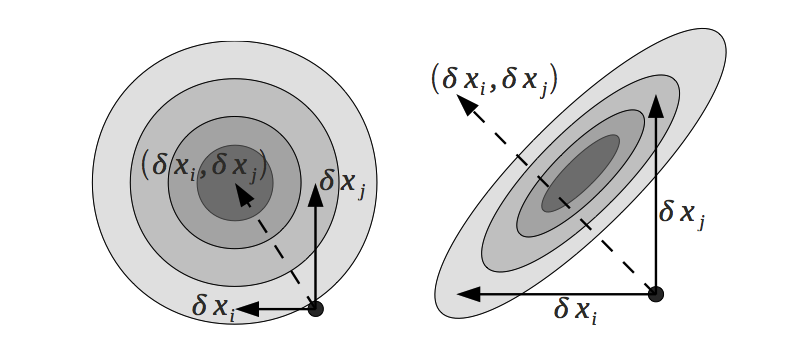
\includegraphics[scale=0.68]{update.png}
\captionof{figure}{Intuition for parallel coordinate descent. Contour plots of two objectives, with darker meaning better. Left: Features are uncorrelated; parallel updates are useful. Right: Features are correlated; parallel updates conflict. $\delta x$ means $\delta \beta$ in our context.}
\end{center}

\begin{center}
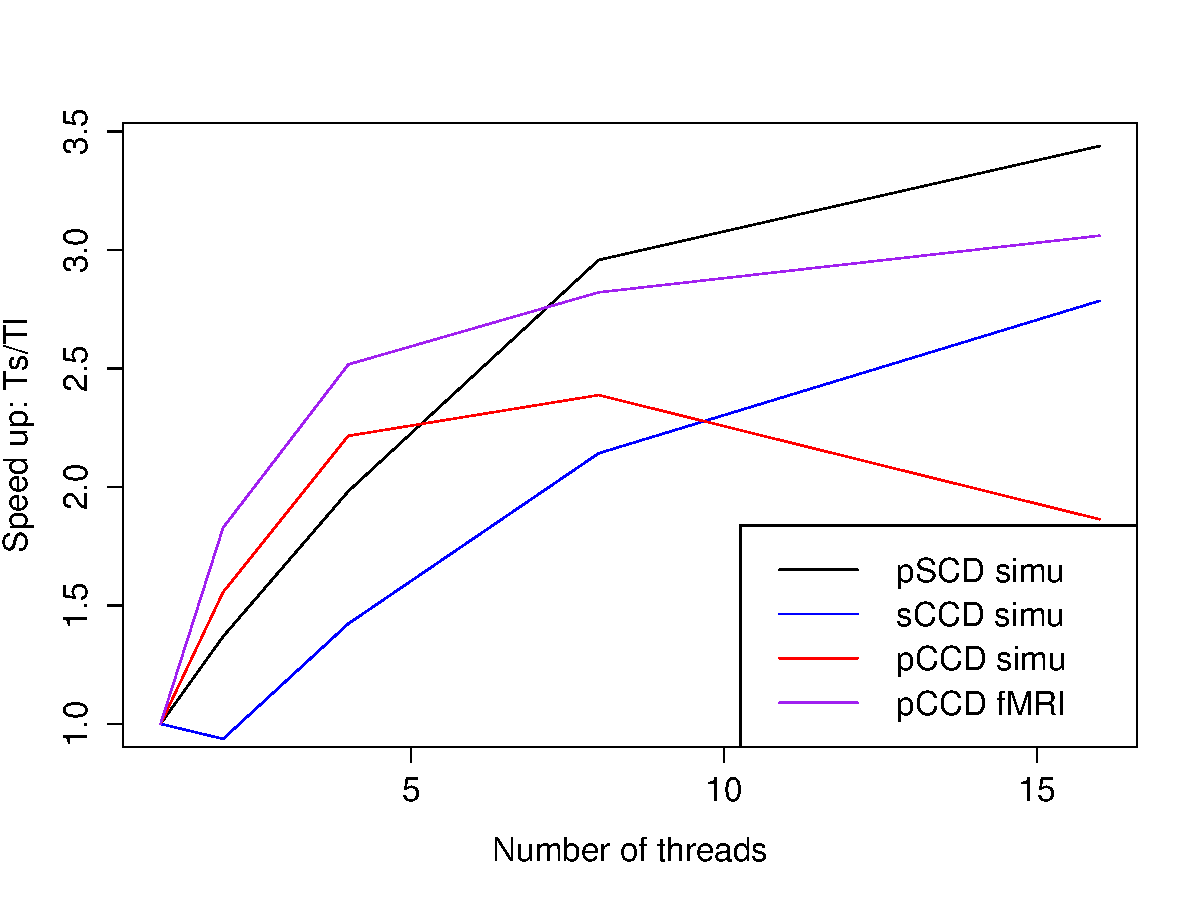
\includegraphics[scale=0.5]{speedup.pdf}
\captionof{figure}{Speed-up comparison between three methods. Black, red, and blue line suggest application to simulated data set. Purple line suggests application to fMRI data set. }
\end{center}

Since pSCD and sCCD failed for fMRI data, in order to compare these methods, they were also applied to a simulated data. The data were simulated by first randomly generating a matrix $X_{2000\times 1000}$ and a vector $\beta_{1000\times 1}$ and setting outcome $Y = X\beta + \epsilon$ where $\epsilon$ is a Gaussian white noise. Then another matrix $Z_{2000\times 1000}$ were generated and column bind with $X$ to serve as the input features. Speed-up curve of these three methods is shown in figure 2, which indicates that pSCD and sCCD do have very good speed-up property when the predictors are not correlated. But pCCD does not speed up very well on simulated data set when using more than $8$ threads, probably due to the fact that the simulated data set is smaller so that there might not be enough work for each thread to amortize the data loading and thread initializing cost.\\

In figure 3, scale-up comparison was made based on running time on simulated data set with varying number of rows but fixed number of columns. As we can see, pSCD has in general better scale-up but the trajectory is some what unpredictable because of its stochastic nature. And sCCD scales a little better than pCCD probably because of the memory access pattern of the implementation of the sparse vector that stores the data.\\

\begin{center}
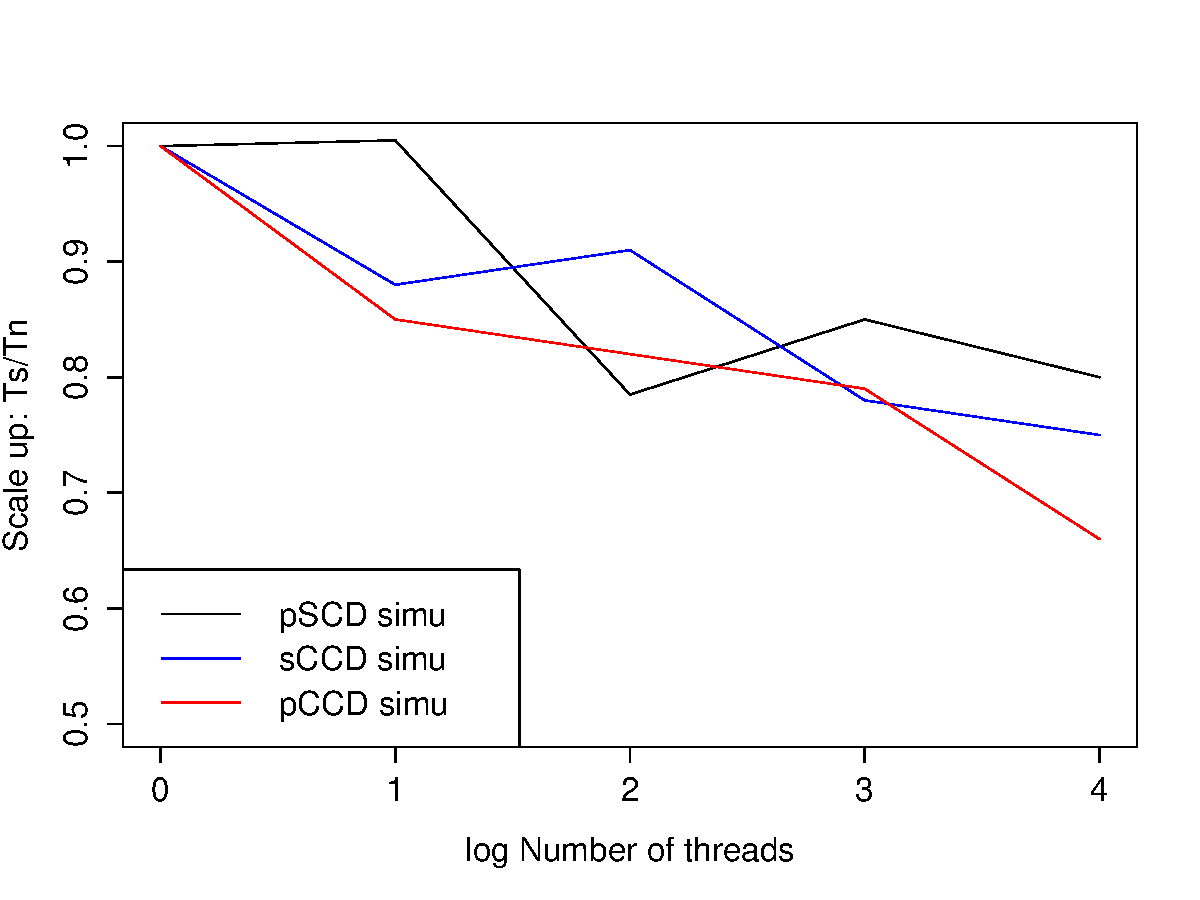
\includegraphics[scale=0.5]{scaleup.pdf}
\captionof{figure}{Scale-up comparison between three methods. Black, red, and blue line suggest application to simulated data set.}
\end{center}

In general, pCCD is the most robust method with good accuracy but almost always the slowest if the other tow also converge. sCCD is subject to large risk of divergence for correlated features, but if features are uncorrelated, it converges faster than pCCD with good accuracy. pSCD cannot deal with correlated features either but if converge, it is always the fastest, however, since it chooses coordinates randomly, by chance, some coordinates are chosen less frequently thus its solution is a worse approximation to the optimum comparing too the other two methods.



\bibliographystyle{plain}
\bibliography{cs420project}
\end{document}